%%%%%%%% ICML 2019 EXAMPLE LATEX SUBMISSION FILE %%%%%%%%%%%%%%%%%

\documentclass{article}

% Recommended, but optional, packages for figures and better typesetting:
\usepackage{microtype}
\usepackage{graphicx}
\usepackage{subfigure}
\usepackage{booktabs} % for professional tables

% hyperref makes hyperlinks in the resulting PDF.
% If your build breaks (sometimes temporarily if a hyperlink spans a page)
% please comment out the following usepackage line and replace
% \usepackage{icml2019} with \usepackage[nohyperref]{icml2019} above.
\usepackage{hyperref}

% Attempt to make hyperref and algorithmic work together better:
\newcommand{\theHalgorithm}{\arabic{algorithm}}

% Use the following line for the initial blind version submitted for review:
%\usepackage{icml2019}

% If accepted, instead use the following line for the camera-ready submission:
\usepackage[accepted]{icml2019}

% The \icmltitle you define below is probably too long as a header.
% Therefore, a short form for the running title is supplied here:
\icmltitlerunning{Learning Optimal Fair Policies}


%Added by Razi 
%+++++++++++++++++++++
\newtheorem{thm}{Theorem}
\usepackage{natbib}
\usepackage{tikz}
\usepackage{epsfig,amssymb,amsmath,ifthen,comment}
\newcommand{\red}{\textcolor{red}}
\newcommand{\blue}{\textcolor{blue}}
\newcommand{\E}{\mathbb{E}}
\DeclareMathOperator{\pa}{pa}
\DeclareMathOperator{\ch}{ch}

\DeclareMathOperator*{\argmax}{arg\,max}
\DeclareMathOperator*{\argmin}{arg\,min}
%+++++++++++++++++++++


\begin{document}

\twocolumn[
%\icmltitle{{\color{blue}Breaking the Cycle Of Injustice Via Learning Fair Policies}}
\icmltitle{Learning Optimal Fair Policies}

% It is OKAY to include author information, even for blind
% submissions: the style file will automatically remove it for you
% unless you've provided the [accepted] option to the icml2019
% package.

% List of affiliations: The first argument should be a (short)
% identifier you will use later to specify author affiliations
% Academic affiliations should list Department, University, City, Region, Country
% Industry affiliations should list Company, City, Region, Country

% You can specify symbols, otherwise they are numbered in order.
% Ideally, you should not use this facility. Affiliations will be numbered
% in order of appearance and this is the preferred way.
\icmlsetsymbol{equal}{*}

\begin{icmlauthorlist}
%\icmlauthor{Aeiau Zzzz}{equal,to}
\icmlauthor{Razieh Nabi}{to}
\icmlauthor{Daniel Malinsky}{to}
\icmlauthor{Ilya Shpitser}{to}
\end{icmlauthorlist}

%\icmlaffiliation{to}{Department of Computation, University of Torontoland, Torontoland, Canada}
\icmlaffiliation{to}{Department of Computer Science, Johns Hopkins University, Baltimore, MD, USA}

%\icmlcorrespondingauthor{Cieua Vvvvv}{c.vvvvv@googol.com}
\icmlcorrespondingauthor{Razieh Nabi}{rnabi@jhu.edu}

% You may provide any keywords that you
% find helpful for describing your paper; these are used to populate
% the "keywords" metadata in the PDF but will not be shown in the document
\icmlkeywords{Fair Policies, Policy Learning, Causal Inference, Mediation Analysis, Algorithmic Fairness, Dynamic Treatment Regimes, Optimal Policies}

\vskip 0.3in
]

% this must go after the closing bracket ] following \twocolumn[ ...

% This command actually creates the footnote in the first column
% listing the affiliations and the copyright notice.
% The command takes one argument, which is text to display at the start of the footnote.
% The \icmlEqualContribution command is standard text for equal contribution.
% Remove it (just {}) if you do not need this facility.

\printAffiliationsAndNotice{}  % leave blank if no need to mention equal contribution
%\printAffiliationsAndNotice{\icmlEqualContribution} % otherwise use the standard text.

\begin{abstract}
Systematic discriminatory biases present in our society influence the way data is collected and stored, the way variables are defined, and the way scientific findings are put into practice as policy. Automated decision procedures and learning algorithms applied to such data may serve to perpetuate existing injustice or unfairness in our society. In this paper, we consider how to make optimal but fair decisions, which ``break the cycle of injustice'' by correcting for the unfair dependence of both decisions and outcomes on sensitive features (e.g., variables that correspond to gender, race, disability, or other protected attributes). 
%In this paper, we consider how to address ``cycles of injustice'' that arise in systems where agents act in an environment to maximize a reward or utility.  In this context, injustice may arise, and persist, if the utility depends in inappropriate ways on a sensitive feature such as race or gender, and agent decisions, possibly in response to this unfair dependence, end up depending on such features in inappropriate ways as well.  We call the unfair dependence of utility on sensitive features \emph{retrospective bias}, and it may arise as a consequence of discriminatory practices or the biased way in which variables are defined or recorded.  We call the unfair dependence of agent decisions on sensitive features \emph{prospective bias}.
We use methods from causal 
%and semiparametric 
inference and constrained optimization to learn optimal policies in a way that addresses 
multiple potential biases which afflict data analysis in sensitive contexts,
%both retrospective bias in the data and prospective bias due to the policy, quantified via 
extending the approach of \citet{NabiShpitser18Fair}.
Our proposal comes equipped with the theoretical guarantee that the chosen fair policy will 
	%``break the cycle of injustice'' in a certain sense: roughly, that the 
induce a joint distribution for new instances
that satisfies given fairness constraints.
%In addition, our methods appropriately address statistical bias due to model misspecification and confounding bias, which are important in the estimation of path-specific causal effects from observational data. 
We illustrate our approach with both synthetic data and real criminal justice data.

%Our proposal aims to provide methods to break this cycle, and make decisions which are both data-driven and sensitive to the aforementioned flaws, so that we do not blindly repeat the mistakes of the past.

%We consider the problem of learning optimal policies from observational data in a way that satisfies certain fairness criteria. The issue of fairness arises where some covariates used in decision making are sensitive features, or are correlated with sensitive features.  \citet{NabiShpitser18Fair} formalized fairness in the context of regression problems as constraining the causal effects of sensitive features along certain disallowed causal pathways.  The existence of these causal effects may be called \emph{retrospective} unfairness in the sense of already being present in the data before analysis begins, and may be the consequence of discriminatory practices or the biased way in which variables are defined or recorded.  In the context of learning policies, what we call \emph{prospective bias}, i.e., the inappropriate dependence of learned policies on sensitive features, is also possible.
\end{abstract}


\section{Introduction} 
%(1) What is the subject of this research, and why is it appropriate for this venue.
Making optimal and adaptive intervention decisions in the face of uncertainty is a central task in precision medicine, computational social science, and artificial intelligence. In healthcare, the problem of learning optimal policies %what we call \emph{optimal policy learning}
is studied under the heading of \emph{dynamic treatment regimes} \cite{Moodie13DTR}.  The same problem is called \emph{reinforcement learning} in artificial intelligence \cite{sutton98reinforcement}, and \emph{optimal stochastic control} \cite{bertsekas96neuro} in engineering and signal processing. In all of these cases, a policy (a function of historical data to some space of possible actions, or a sequence of such functions) is chosen to maximize some pre-specified outcome quantity, which might be abstractly considered a \emph{utility} (or \emph{reward} in reinforcement learning). Increasingly, ideas from optimal policy learning % that originated in medicine or computer science
are being applied in new contexts. In some areas, particularly socially-impactful settings like criminal justice, social welfare policy, hiring, and personal finance, it is essential that automated decisions respect principles of fairness since the relevant data sets include potentially sensitive attributes (e.g., race, gender, age, disability status) and/or features highly correlated with such attributes, so ignoring fairness considerations may have socially unacceptable consequences.  A particular worry in the context of automated sequential decision making is ``perpetuating injustice,'' i.e., when maximizing utility maintains, reinforces, or even introduces unfair dependence between sensitive features, decisions, and outcomes. Though there has been growing interest in the issues of fairness in machine learning \cite{pedreshi08discrimination,feldman15certifying,hardt16equality,kamiran13quantifying,corbett2017algorithmic,jabbari16fair,kusner17counterfactual,zhang18fairness,mitchell18speak,Zhang17causal}, so far methods for 
%{\color{blue}making sequential decisions fairly, and in particular escaping above cycles of injustice}
optimal policy learning subject to fairness constraints
have not been well-explored. %are underinvestigated.

%(2) Concrete motivating example
As a motivating example, we consider a simplified model for a children's welfare screening program, recently discussed in \cite{chouldechova2018case, Hurley18child}. A hotline for child abuse and neglect receives many thousands of calls a year, and call screeners must decide on the basis of calculated risk estimates what action to take in response to any given call, e.g., whether or not to follow up with an in-person visit from a caseworker. The idea is that only cases with substantial potential risk to the child's welfare should be prioritized. The information used to determine the calculated risk level and thereby the agency's action includes potentially sensitive features, such as race and gender, as well as a myriad of other factors such as perhaps whether family members receive public assistance, have an incarceration history, record of drug use, and so on. Though many of these factors may be predictive of subsequent negative outcomes for the children, there is a legitimate worry that both risk calculations and policy choices based on them may depend on sensitive features in inappropriate ways, and thereby lead
 %that some policy choices lead
to unfair racial disparities in the distribution of families investigated, and perhaps separated, by child protective services.

%(3) Why the problem is interesting/difficult
Learning high-quality policies that satisfy fairness constraints is difficult due to the fact that multiple sources of bias may occur in the problem simultaneously. One kind of bias, which we call \emph{retrospective bias}, has its origin in the historical data used as input to the policy learning procedure.  This data may reflect various systematic disparities and discriminatory historical practices in our society, including prior decisions themselves based on poor data.  Algorithms trained on such data can %reinforce
maintain these inequities.  Furthermore, decision making algorithms may suffer from what we call \emph{prospective} sources of bias. For instance, suppose the functional form of the chosen decision rule explicitly depends on sensitive features in inappropriate ways.  In that case, making decisions based on the new decision rule may perpetuate existing disparities or even introduce disparities that were previously absent.  Avoiding this sort of bias may involve imposing non-trivial restrictions on the policy learning procedure. Finally, learning high-quality policies from observational data requires dealing with \emph{confounding bias}, where associations between decision and reward cannot be used directly to assess decision quality due to the presence of confounding variables, as well as \emph{statistical bias} due to the reliance on misspecified statistical models.  Policy learning algorithms that respect fairness constraints must address all of these sources of bias.

%(4) What are our contributions.
In this paper, we use tools from mediation analysis and causal inference to formalize fairness criteria as constraints on certain impermissible causal pathways from sensitive features to actions or outcomes \cite{NabiShpitser18Fair}. Moreover, we describe how all the aforementioned biases can be addressed by a novel combination of methods from causal inference, constrained optimization, and semiparametric statistics. Our main theoretical result illustrates in what sense enacting fair policies can ``break the cycle of injustice'':
we show how to learn policies such that the joint distribution induced by these policies (in conjunction with reward/utility mechanisms outside the policy-maker's control) will satisfy specified fairness constraints while remaining ``close'' to the generating distribution.
%which satisfies the specified fairness constraints.
To our knowledge, this paper constitutes the first attempt to integrate algorithmic fairness and policy learning with the possible exception of \citet{jabbari16fair}, which addressed what we call prospective bias in the context of Markov Decision Processes. 

%(5) outline 
%\red{May need to revise!}
%The paper is organized as follows. We first fix our notation and give a short introduction to causal inference and mediation analysis, which will be necessary to formally define our approach to fair decision making, and review common techniques for learning optimal policies. We then describe in general how to impose fairness constraints for the purpose of policy learning. Moving forward, we present our procedure to learn optimal fair policies from data and discuss a number of distinct approaches to solving the relevant constrained optimization problems. 
%%We present a number of experiments on synthetic and real data. Our conclusions are in Section 6.
%We present a number of experiments on synthetic and real data in the experimental section followed by our final conclusions.  
%%We illustrate our framework via experiments on real datasets in the experimental section followed by additional discussion and final conclusions.

To precisely describe our approach, we must introduce some necessary concepts and tools from causal inference and policy learning. Then, we summarize the perspective on algorithmic fairness in prediction problems from \citet{NabiShpitser18Fair}, and adapt this framework to learning optimal fair policies. We illustrate our proposal via experiments on synthetic and real data.

\section{Notation and preliminaries} 
\label{sec:prelim}

Consider a multi-stage decision problem with $K$ pre-specified decision points, indexed by $k = 1, \ldots, K$.  Let $Y$ denote the final outcome of interest and $A_k$ denote the action made (treatment administered) at decision point $k$ with the finite state space of ${\cal A}_k$. Let $X$ denote the available information prior to the first decision, and $Y_k$ denote the information collected between decisions $k$ and $k+1$, ($Y \equiv Y_{K}$). $\overline{A}_k$ represents all treatments administered from time $1$ to $k$; likewise for $\overline{Y}_k$. We combine the treatment and covariate history up to treatment decision $A_k$ into a history vector $H_k$. The state space of $H_k$ is denoted by ${{\cal H}_k}$. Note that while our proposal in this paper applies to arbitrary state spaces,
% though
we
%mostly
present examples with continuous outcomes and binary decisions for simplicity.

The goal of policy learning is to find
%We are interested in learning
policies that map vectors in ${\cal H}_k$ to values in ${\cal A}_k$ (for all $k$)
%to
that
maximize the expected value of outcome $Y$.
%To do so we must reason counterfactually, as is common in causal inference.
In offline settings, where exploration by direct experimentation is impossible, finding such policies requires reasoning counterfactually, as is common in causal inference.
The value of $Y$ under an assignment of value $a$ to variable $A$
%$A=a$
is called a \emph{potential outcome} variable, denoted $Y(a)$. In causal inference, quantities of interest are defined as functions of potential outcomes (also called counterfactuals). Estimating these functions  from observational data is a challenging task, and requires assumptions linking potential outcomes to the data actually observed. Our assumptions can be formally represented using \textit{causal graphs}.  In a directed acyclic graph (DAG), nodes correspond to random variables, and directed edges represent direct causal relationships. As an example, consider the single treatment causal graph of Fig. \ref{fig:triangle}(a). $X$ is a direct cause of $A$, and $A$ is both a direct cause of $Y$ as well as an indirect cause of $Y$ through $M$. A variable like $M$ which lies on a causal pathway from $A$ to $Y$ is called a \textit{mediator}.
%A variable which is a common cause of both $A$ and $Y$ is called a \textit{confounder} for the effect of $A$ on $Y$.
For more details on causal graphical models see, e.g., \citet{spirtes01causation} and \citet{pearl09causality}. In what follows let $Z$ denote the full vector of observed variables in the causal model, e.g., $Z = (Y,M,A,X)$ in our Fig. \ref{fig:triangle}(a).
%One such assumption is \textit{consistency}, stating that $Y = Y(a)$ if $A=a$. %took this out because we don't give a laundry list of assumptions anywhere, just draw graphs.

A causal parameter is said to be \emph{identified} in a causal model if it is a function of the observed data distribution $p(Z)$. In causal DAGs, distributions of potential outcomes are identified by the \emph{g-formula}. For background on general identification theory, see \citet{shpitser18identification}.
%Distributions of potential outcomes $p(\{ Z \setminus A \}(a))$, for any subset $A$ of $Z$, are identified by the \emph{g-formula}:
%{\small
%\begin{align}
%$p(\{ Z \setminus A \}(a)) =
%\!\!\!
%\prod_{V \in \{ Z \setminus A \}}
%\left.
%\!\!\!
%p(V | \pa_{\cal G}(V)) \right|_{A=a}$,
%\label{eqn:g}
%\end{align}
%}\noindent
%where $\pa_{\cal G}(V)$ is the set of direct causes of $V$ in DAG ${\cal G}$, called the \emph{parent} set. 
As an example, the distribution of $Y(a)$ in the DAG in Fig.~\ref{fig:triangle}(a) %is defined to be $Y(a,M(a,W),W)$, 
%and its distribution
is identified by $\sum_{X,M} p(Y | a,M,X) p(M | a,X) p(X)$.
%{\color{blue}Expectations over such counterfactual distributions are used to define causal effects such as the \emph{average causal effect (ACE):} $\mathbb{E}[Y(a)] - \mathbb{E}[Y(a')]$.}
Note that some causal parameters may be identified even in causal models with hidden (``latent'') variables, typically represented by acyclic directed mixed graphs (ADMGs) \citep{shpitser18identification}. Though we do not apply our methods to hidden variable models here, the general approach and many of the specific learning strategies we propose are applicable in contexts with hidden variables, so long as the relevant parameters are identified.

In our sequential setting,
% if we wish to evaluate the outcome had a sequence $\overline{a}_K$ of decisions been made, the relevant counterfactual is
$Y(\overline{a}_K)$ represents the response $Y$ had the fixed treatment assignment strategy $\overline{A}_K = \overline{a}_K$ been followed, possibly contrary to fact.  The contrast %, in expectation of $Y(\overline{a}_K)$ and $Y(\overline{a}'_K)$,
$\E[Y(\overline{a}_K)] - \E[Y(\overline{a}'_K)]$, where $\overline{a}_K$ is the treatment history of interest and $\overline{a}'_K$ is the reference treatment history, quantifies the \emph{average causal effect} of $\overline{a}_K$ on the outcome $Y$.
%In this paper, we are concerned with setting $\overline{a}_K$ dynamically based on observed history.

\subsection*{Mediation and path-specific analysis}

%{\color{blue}Our goal is to use causal reasoning to find \emph{dynamic} treatment assignment strategies for $\overline{A}_K$ that satisfy fairness constraints.  Following \citet{NabiShpitser18Fair}, these constraints entail the absence of dependence of variables on the sensitive feature along inadmissible causal pathways.  We now introduce mediation analysis to quantify these constraints.}

%%(5) mediation analysis
%An important task in causal inference is to understand the mechanisms by which treatments influence outcomes.
%% In a single decision point problem,
%A common approach to understanding mechanisms is \textit{mediation analysis}, wherein
One way to understand the mechanisms by which treatments influence outcomes is via mediation analysis.
The simplest type of mediation analysis
%one
decomposes the causal effect of $A$ on $Y$ into a \textit{direct effect} and an \textit{indirect effect} mediated by a third variable. Consider the graph in Fig \ref{fig:triangle}(a): the direct effect corresponds to the path $A \rightarrow Y$, and indirect effect corresponds to the path through $M$: $A \rightarrow M \rightarrow Y$. In the potential outcome notation, the direct and indirect effects can be defined using nested counterfactuals such as $Y(a, M(a'))$ for $a, a' \in \cal A$, which denotes the value of $Y$ when $A$ is set to $a$ while $M$ is set to whatever value it would have attained had $A$ been set to $a'$. Under certain identification assumptions discussed by \citet{pearl01direct}, the distribution of $Y(a, M(a'))$ (and thereby direct and indirect effects) can be nonparametrically identified from observed data by the following formula:
%{\small
%\begin{align}
$p(Y(a, M(a')) = \sum_{X, M} p(Y \mid a, X, M) p(M \mid a', X) p(X)$.
%\end{align}
%}
More generally, when there are multiple pathways from $A$ to $Y$ one may define various \textit{path-specific effects} (PSEs), which under some assumptions may be nonparametrically identified by means of the \textit{edge g-formula} provided in \citet{shpitser15hierarchy}.  We define a number of PSEs relevant for our examples below.  For a general definition, see \citet{shpitser13cogsci}.


\subsection*{Policy counterfactuals and policy learning}
\label{sec:policy}

%{\color{blue}We now describe methods to offline policy learning developed in causal inference, as a prelude to describing our approach to making these methods fair.}
Let $f_A = \{f_{A_1}, \ldots, f_{A_K} \}$ be a sequence of decision rules. 
At the $k$th decision point, the $k$th rule $f_{A_k}$ maps the available information prior to the $k$th treatment decision $H_k$ to treatment decision $a_k$, i.e.\ $f_{A_k}: {{\cal H}_k} \mapsto {{\cal A}_k}$.
Given $f_A$ we define the counterfactual response of $Y$ had $A$ been assigned according to $f_A$,
or $Y(f_A)$, by the following recursive definition \citep[cf.][]{robins04SNMM,thomas13swig}:
{\small
\begin{align*}
Y\big(
\big\{ f_{A_k}\big(H_k(f_{A})\big): A_k \in \pa_{\cal G}(Y)\cap A \big\},
\big\{ \pa_{\cal G}(Y) \setminus A \big\}(f_A)
\big).
%\label{eqn:rec-sub-f}
\end{align*} 
}% 
In words: the potential outcome $Y$ had any parent of $Y$ that is in $A$ been set to $f_A$ in response to counterfactual history $H_k$ up to $k$, where this history behaves as if $A$ were set to $f_A$ \textit{and} any parent of $Y$ that is not in $A$, behaves as if $A$ were set to $f_A$. 

Under a causal model associated with the DAG $\cal G$, the distribution $p(Y(f_A))$, is identified by the following generalization of the g-formula:
{\scriptsize
\begin{align*}
\sum_{Z \setminus \{Y, A \}}   \prod_{V \in Z \setminus A}
p\big(V | \{ f_{A_k}(H_k): A_k \in \pa_{\cal G}(V) \cap A \}, \pa_{\cal G}(V) \setminus A \big).
%\label{eqn:g-f}
\end{align*}
}%
%{\color{blue}
%{\small
%\begin{align*}
%\sum_{Z \setminus Y, A} & \ \prod_{V \in Z \setminus A}
%p\big(V | \{ f_{A_i}(H_i): A_i \in \pa_{\cal G}(V) \cap A \}, \pa_{\cal G}(V) \setminus A \big)\\
%& \ \prod_{A_i \in A} \tilde{p}_i(A_i | H_i),
%%\label{eqn:g-f}
%\end{align*}
%}
%where $\tilde{p}(a_i | H_i) = 1$ if $f_{A_i}(H_i) = a_i$.
%}
As an example, $Y(a = f_A(X))$ in Fig.~\ref{fig:triangle}(a) is defined as $Y(a=f_A(X), M(a=f_A(X),X), X)$, 
and its distribution is identified as
$\sum_{x,m} p(Y | a=f_A(x),M=m,X=x) p(M | a=f_A(x),X=x) p(X=x)$.
%{\color{blue}
%$\sum_{x,m} p(Y | \tilde{a},m,x) p(m | \tilde{a},x) \tilde{p}(\tilde{a} | x) p(x)$, with $\tilde{p}(a | x) = 1$ if %$f_A(x) = a$.
%}

Given an identified response to a fixed set of policies $f_A$, we consider search for the optimal policy set $f^*_A$, defined to be one that maximizes $\E[Y(f_A)]$.
%a common goal is to learn the set of \emph{optimal} policies, where the optimal policy set $f^*_A$ is defined to be one that maximizes
%$\E[Y(f_A)]$.
Since $Y(f_A)$ is a counterfactual quantity, validating the found set of policies is difficult given only retrospective data, with statistical bias due to model misspecification being a particular worry.  This stands in contrast with online policy learning problems in reinforcement learning, where new data under any policy may be generated and validation is therefore automatic. Partly in response to this issue, a set of orthogonal methods for policy learning have been developed that model different parts of the observed data likelihood function.
%Because of the difficulty of validating the quality of learned policies, a
Q-learning, value search, and g-estimation are common methods used in dynamic treatment regimes literature for learning optimal policies \cite{Moodie13DTR}. We defer detailed descriptions to later in the paper and the supplement.

\begin{figure*}
\begin{center}
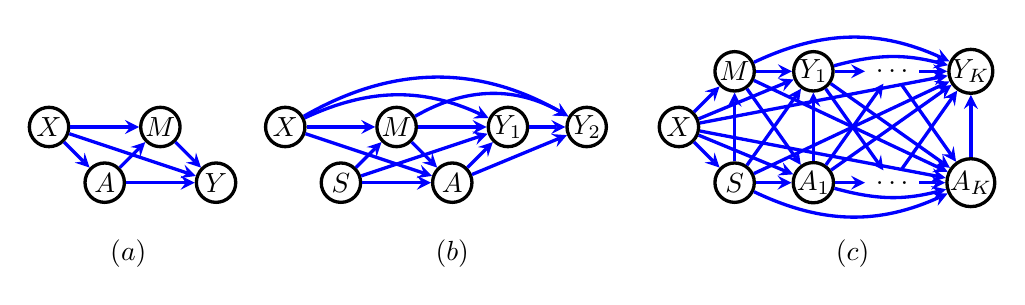
\begin{tikzpicture}[>=stealth, node distance=1.0cm]
    \tikzstyle{format} = [draw, very thick, circle, minimum size=5.0mm,
	inner sep=0pt]
	\begin{scope}
		\path[->, very thick]
			node[format] (c) {$X$}
			node[format, below right of=c] (a) {$A$}		
			node[format, above right of=a] (m) {$M$}
			node[format, below right of=m] (y) {$Y$}
			(c) edge[blue] (a)
			(a) edge[blue] (y)
			(a) edge[blue] (m)
			(m) edge[blue] (y)
			(c) edge[blue] (m)
			(c) edge[blue] (y)
			node[below of=a, yshift=0.1cm, xshift=0.3cm] (l) {$(a)$}	
			;
	\end{scope}
	
	\begin{scope}[xshift=3.0cm] %[xshift=2.2cm]
		\path[->, very thick]
			node[format] (x) {$X$}
			node[format, below right of=x] (s) {$S$}
			node[format, above right of=s] (m) {$M$}
			%node[format, gray, above right of=m] (u) {$U$}
			node[format, below right of=m] (a) {$A$}
			node[format, above right of=a] (y) {$Y_1$}
			node[format, right of=y] (y2) {$Y_2$}
			%  (w) edge[blue] (a)
			(s) edge[blue] (a)
			(s) edge[blue] (m) 
			(m) edge[blue] (a)
			(x) edge[blue] (m)
			(x) edge[blue] (a)
			(a) edge[blue] (y)
			(m) edge[blue] (y)
			(s) edge[blue] (y) 
			(x) edge[blue, bend left=25] (y)
%			(u) edge[red] (m)
%			(u) edge[red] (y)
			(x) edge[blue, bend left] (y2)
			(a) edge[blue] (y2)
			(y) edge[blue] (y2)
			(m) edge[blue, bend left] (y2)
			 
			node[below of=a, yshift=0.1cm, xshift=0.0cm] (l) {$(b)$}
		;
	\end{scope}

	\begin{scope}[xshift=8.0cm] %[xshift=11.5cm] %[xshift=2.2cm]
	\path[->, very thick]
%	node[format] (x) {$X$}
%	node[format, below right of=x] (s) {$S$}
%	node[format, above right of=s] (m) {$M$}
%	node[format, below right of=m] (a1) {$A_1$}
%	node[format, above right of=a1] (y1) {$Y_1$}
%	node[ below right of=y1] (dots1) {$\ldots$}
%	node[ above right of=dots1] (dots2) {$\ldots$}
%	node[format, below right of=dots2] (aK) {$A_K$}
%	node[format, above right of=aK] (yK) {$Y_K$}
	
	node[format] (x) {$X$}
	node[format, below right of=x] (s) {$S$}
	node[format, above right of=x] (m) {$M$}
	node[format, right of=s] (a1) {$A_1$}
	node[format, right of=m] (y1) {$Y_1$}
	node[  right of=a1] (dots1) {$\ldots$}
	node[  right of=y1] (dots2) {$\ldots$}
	node[format,  right of=dots1] (aK) {$A_K$}
	node[format,  right of=dots2] (yK) {$Y_K$}
	
	(y1) edge[blue] (dots2)
	(a1) edge[blue] (dots2)
	%(s) edge[blue, bend right=52] (dots2)
	%(m) edge[blue, bend left=20] (dots2)	
	%(x) edge[blue, bend left=20] (dots2)

	(y1) edge[blue] (dots1)
	(a1) edge[blue] (dots1)
	%(m) edge[blue, bend left=0] (dots1)
	%(s) edge[blue, bend right=30] (dots1)
	%(x) edge[blue, bend left=0] (dots1)

	(dots1) edge[blue, bend left=0] (aK)
	(dots2) edge[blue, bend left=0] (aK)
	(m) edge[blue, bend left=0] (aK)
	(y1) edge[blue] (aK)
	(a1) edge[blue, bend right=15] (aK)
	(s) edge[blue, , bend right=25] (aK)
	(x) edge[blue, bend left=0] (aK)

	(dots1) edge[blue] (yK)
	(dots2) edge[blue] (yK)
	(m) edge[blue, bend left=25] (yK)
	(x) edge[blue, bend left=0] (yK)
	(y1) edge[blue, bend left=15] (yK)
	(s) edge[blue, bend left=0] (yK)
	(a1) edge[blue] (yK)
	(aK) edge[blue] (yK)

	%(s) edge[blue, bend right=0] (yK)

	(x) edge[blue] (s)

	(s) edge[blue] (a1)
	(m) edge[blue] (a1)
	(x) edge[blue] (a1)

	(s) edge[blue] (m)
	(x) edge[blue] (m)

	(a1) edge[blue] (y1)
	(m) edge[blue] (y1)
	(x) edge[blue, bend left=0] (y1)
	(s) edge[blue] (y1)

	node[below of=a1, yshift=0.1cm, xshift=0.5cm] (l) {$(c)$}
	;
	\end{scope}

\end{tikzpicture}
\end{center}
\caption{(a) A simple causal DAG, with a single treatment $A$, a single outcome $Y$, a vector $X$ of baseline variables, and a single mediator $M$.
(b) A causal DAG corresponding to our (simplified) child welfare example with baseline factors $X$, sensitive feature $S$, action $A$, vector of mediators (including e.g.\ socioeconomic variables, histories of drug treatment) $M$, an indicator $Y_1$ of whether a child is separated from their parents, and an indicator of child hospitalization $Y_2$. (d) A multistage decision problem, which corresponds to a complete DAG over vertices $X,S,M,A_1,Y_1,\cdots,A_K,Y_K$.
}
\label{fig:triangle}
\end{figure*} 

%\section{Making decisions in a fair world}
\section{From fair prediction to fair policies}
\label{sec:fairpolicy}

%\section*{Algorithmic Fairness And Policy Learning} 
%(9) literature on fairness

\citet{NabiShpitser18Fair} argue that fair inference for prediction requires imposing hard constraints on the prediction problem, in the form of restricting certain path-specific effects. We adapt this approach to optimal sequential decision-making.
%We generalize the method for satisfying fairness constraints in prediction problems developed in \citet{NabiShpitser18Fair} to policy learning problems for optimal sequential decision making.  Specifically, we learn policies in such a way that the joint distribution resulting from following learned policies, and the environment assigning reward as a result, such as
%$p(Y | \tilde{a},m,x) p(m | \tilde{a},x) \tilde{p}(\tilde{a} | x) p(x)$ in the previous section,
%do not contain effects of sensitive features along certain impermissible causal pathways.
%in the data-generating process {\color{blue}and the , and then performing inference from this restricted model.
A feature of this approach is that the relevant restrictions are user-specified and context-specific; thus we will generally require input from policymakers, legal experts, bioethicists, or the general public in applied settings. Which pathways may be considered impermissible depends on the domain and the semantics of the variables involved. We do not defend this perspective on fairness here for lack of space; please see \citet{NabiShpitser18Fair}
% and \citet{pearl09causality}
for more details.

%There has recently been an explosion of interest in fairness in machine learning, particularly in the context of prediction and classification algorithms \cite{pedreshi08discrimination,feldman15certifying,hardt16equality,kamiran13quantifying,
%corbett-davies17algorithmic,jabbari16fair,kusner17counterfactual,zhang18fairness,mitchell18speak}.  Many definitions of fairness have been proposed in the literature

%--- prior stuff.
We summarize the proposal from \citet{NabiShpitser18Fair} with a brief example, inspired by the aforementioned child welfare case. Consider a simple causal model for this scenario, shown in Fig.\ 1(b). Hotline operators receive thousands of calls per year, and must decide on an action $A$ for each call, e.g., whether or not to send a caseworker. These decisions are made on the basis of a (high-dimensional) vectors of covariates $X$ and $M$, as well as possibly sensitive features $S$, such as race. $M$ consists of mediators of the effect of $S$ on $A$. $Y_1$ corresponds to an indicator for whether the child is separated from their family by child protective services, and $Y_2$ corresponds to child hospitalization (presumably attributed to domestic abuse or neglect). The observed joint distribution generated by this causal model would be $p(Y_1,Y_2,A,M,S,X)$. The proposal from \citet{NabiShpitser18Fair} is that fairness corresponds to the impermissibility of certain path-specific effects, and so fair inference requires decisions to be made from a counterfactual distribution $p^*(Y_1,Y_2,A,M,S,X)$ which is ``nearby'' to $p$ (in the sense of minimal Kullback-Leibler divergence) but where these PSEs are constrained to be zero. They call $p^*$ the distribution generated by a ``fair world.''

Multiple fairness concerns have been raised by experts and advocates in discussions of the child protection decision-making process \cite{chouldechova2018case, Hurley18child}. For example, it is clearly impermissible that race has any direct effect on the decision made by the hotline screener, i.e., that all else being held fixed, members from one group have a higher probability of being surveilled by the agency. However, it is perhaps permissible that race has an indirect effect via some mediated pathway, e.g., if race is associated with some behaviors or features which themselves ought to be taken into consideration by hotline staffers, because they are predictive of abuse. If that's true, then $S \rightarrow A$ would be labeled an impermissible pathway whereas $S \rightarrow M \rightarrow A$ (for some $M$) would be permissible. Similarly, it would be unacceptable if race had an effect on whether children are separated from their families; arguably both the direct pathway $S \rightarrow Y_1$ and indirect pathway though hotline decisions $S \rightarrow A \rightarrow Y_1$ should be considered impermissible. Rather than defend any particular choice of path-specific constraints, we note that the framework outlined in \citet{NabiShpitser18Fair} can flexibly accommodate any set of given constraints, as long as the PSEs are identifiable from the observed distribution.

%A lot of interest in literature on fairness are related to regression and classification algorithms and there are many proposals on defining fairness. They can be categorized into associational and causal notions of fairness, \citep{NabiShpitser18Fair, Zhang17causal, Kilbertus17fair, Kusner17fair, hardt16equality}. We believe, any approach that relies on associative measures of fairness will do an intuitively wrong thing in scenarios where the sensitive feature is not randomly assigned, like gender, but instead exhibits spurious correlations with the outcome through other possibly unobserved features. An example of such a feature is prior conviction status (certain types of decisions, such as hiring, forbid discrimination on this feature). 

%Even in cases where the sensitive feature is randomized, seemingly sensible definitions tend to be overly restrictive. Consider the hiring example where potential discrimination is with respect to gender (a variable that is randomized at birth). It makes intuitive sense to say that job applicants' gender should not directly influence the hiring decision, but may influence the hiring decision indirectly, via secondary applicant characteristics important for the job, and correlated with gender. In this example, discrimination intuitively corresponds to a part of the causal relationship between gender and the hiring decision. We adapt the notion of fairness in \citep{NabiShpitser18Fair} that links discrimination to presence of effect along impermissible causal pathways.  

%Given $p$ and identifying functionals for the relevant PSEs, \citep{NabiShpitser18Fair} construct $p^*$ via constrained maximum likelihood estimation.
\subsection{Inference in a nearby ``fair world''}

We now describe the specifics of the proposal.
We assume the data is generated according to some (known) causal model, with observed data distribution $p(\cdot)$, and that we can characterize the fair world by a fair distribution $p^*(\cdot)$ where some set of pre-specified PSEs are constrained to be zero, or within a tolerance range. 
Without loss of generality we can assume the utility variable $Y$ is some deterministic function of $Y_1$ and $Y_2$ (i.e., $Y \equiv u(Y_1,Y_2)$) and thus use $Y$ in place of $Y_1$ and $Y_2$ in what follows.
% (see Fig.\ 1(c)).
Then $Z = (Y,X,S,M,A)$ in our child welfare example. For the purposes of illustration, assume the following two PSEs are impermissible:
PSE$^{sa}$, corresponding to the direct effect of $S$ on $A$ and defined as $\E[A(s,M(s'))] - \E[A(s')]$, and
PSE$^{sy}$, corresponding to the effect of $S$ on $Y$ along the edge $S \to Y$, and the path $S \to A \to Y$ and defined as $\E[Y(s, A(s,M(s')), M(s'))] - \E[Y(s')]$.
%In a multi-stage version of this decision problem, the relevant decision variables, multiple outcomes, and so on would all be collected in $Z$.

If the PSEs are identified under the considered causal model, they can be written as functions of the observed distribution. For example, the unfair PSE of the sensitive feature $S$ on outcome $Y$ in our child welfare example may be written as a functional PSE$^{sy} = g_1(Z) \equiv g_1(p(Y, X, S, M, A))$. Similarly the unfair PSE of $S$ on $A$ is PSE$^{sa}$ $= g_2(Z) \equiv g_2(p(Y, X, S, M, A))$. Generally, given a set of identified PSEs $g_j(Z)$ $\forall j \in \{ 1,..., J \}$ and corresponding tolerated lower/upper bounds $\epsilon_j^-, \epsilon_j^+$, the fair distribution $p^*(Z)$ is defined:
{\small
	\begin{align}
	p^*(Z) &\equiv \arg \min_{q} \hspace{0.1cm} D_{KL}(p||q) \nonumber \\
	\text{ subject to} \hspace{0.2cm} & \epsilon_j^- \leq g_j(Z) \leq \epsilon_j^+, \hspace{0.2cm} \forall j \in \{ 1,...,J \},
	\label{eqn:p-star}
	\end{align}
}%
where $D_{KL}$ is the KL-divergence and $J$ is the number of constraints.\footnote{Note that in our examples $J$ will typically be $K+1$, i.e., one constraint for the $S$ to $Y$ paths and one constraint for each set of paths from $S$ to $A_k$. We allow for $J$ constraints in general to accommodate more complex settings (e.g., where there are multiple sensitive features, multiple outcomes, or a different set of pathways are constrained).} In finite sample settings, \citet{NabiShpitser18Fair} propose solving the following constrained maximum likelihood problem:
{\small
\begin{align}
\widehat{\alpha} &= \arg \max_{\alpha} \hspace{0.1cm} {\cal L}(Z; {\alpha}) \nonumber \\
\text{ subject to} \hspace{0.2cm} & \epsilon_j^- \leq \widehat{g}_j(Z) \leq \epsilon_j^+, \hspace{0.2cm} \forall j \in \{ 1,...,J \},
 \label{eqn:c-mle}
\end{align}
}%
where $\widehat{g}_j(Z)$ are estimators for the chosen PSEs and ${\cal L}(Z; \alpha)$ is the likelihood function. The most relevant bounds in practice are $\epsilon_j^- =  \epsilon_j^+ = 0$.

Given an approximation of $p^*$ learned in this way, \citet{NabiShpitser18Fair} transform regression problems originally defined on $p$ into regression problems on $p^*$.
In other words, instead of learning a regression function $\mathbb{E}[Y \mid M, A, S, X]$ on the observed data distribution $p(Z)$, they approximate the fair distribution $p^*(Z)$ by constrained maximum likelihood and classify new instances using the constrained model. As we discuss in more detail later, \citet{NabiShpitser18Fair} choose to average over certain variables to accomodate the fact that new instances are generated from $p$ rather than $p^*$.

%a new distribution $p^*(Z)$ was constructed where for some $W \subset Z$, $p^*(W) = p(W)$.  The regression function learned was then $\mathbb{E}^*[Y | W]$, and new instances $M_i, A_i, S_i, X_i$ were classified based only on features in $W$ with others ``averaged over'' with respect to $p^*$.  In this way, the entire regression problem was rephrased to apply on $p^*(Z)$, where fairness constraints held by construction, rather than $p^*(Y | M,A,S,X) p(M, A, S, X)$ (the distribution involved if all features $M_i, A_i, S_i, X_i$ of a new instance were used), where fairness constraints would not be guaranteed to hold.  The choice of $W$ and $Z \setminus W$ was guided by the estimator used to obtain the PSEs.  For instance, if the inverse probability weighted (IPW) estimator was used which used models $A$ and $M$, then $Z \setminus W = \{ A, M \}$.


\subsection{Fair decision-making}

%However, doing so requires modifying the method of out of sample prediction, since new instances will be drawn from the observed distribution $p(Z)$ rather than the fair distribution $p^*(Z)$.
%Following \citep{NabiShpitser18Fair},
In the sequential decision setting, there are multiple complications.
%We require constraints on multiple pathways, must find an optimal policy while respecting those constraints, and endeavour to induce a distribution on the system that satisfies these fairness criteria even despite mechanisms that are outside the control of the policy-maker.
In particular, we aim to learn high-quality policies while simultaneously making sure that the joint distribution induced by the 
policy satisfies our fairness criteria, potentially involving constraints on multiple causal pathways.  This problem must be solved in settings where distributions of some variables, such as outcomes, are not under the policy-maker's control.  Finally, we must show that if the learned policy is adapted to new instances (drawn from the original observed distribution) in the right way, then these new instances combined with the learned policy, constrained variables, and variables outside our control, together form a joint distribution where our fairness criteria remain satisfied.
%We adapt this proposal to our sequential decision setting as follows. 


Consider a $K$-stage decision problem given by a DAG where every vertex pair is connected, and with vertices in a topological order $X, S, M, A_1, Y_1, \ldots, A_K, Y_K$. See Fig.\ 1(c). Note that the setting where $S$ can be assumed exogenous is a special case of this model with missing edge between $X$ and $S$. Though we only assume a single set of permissible mediators $M$ here, at the expense of some added cumbersome notation all of the following can be extended to the case where there are distinct sets of mediators $M_1, \ldots, M_K$ preceding every decision point. (We extend the results below to that setting in the Supplement.)
We will consider the following PSEs as inadmissible: PSE$^{sy}$, representing the effect of $S$ on $Y$ along all paths \emph{other than} the paths of the form $S \to M \to \ldots \to Y$; and PSE$^{sa_k}$, representing the effect of $S$ on $A_k$ along all paths \emph{other than} the paths of the form $S \to M \to \ldots \to A_k$. That is, we consider \emph{only} pathways connecting $S$ and $A_k$ or $Y$ through the allowed mediators $M$ to be fair. 
%The setting where there are no permissible mediators is of course a special case.
In this model, these PSEs are identified by \cite{shpitser13cogsci}:
{\small
	\begin{align*}
	\text{PSE}^{sy} 
	&= \E[Y(s,M(s'))] - \E[Y(s')] \\ 
	= \sum_{X,M} &\{ \E[Y | s,M,X] - \E[Y | s',M,X] \} p(M | s',X) p(X)\\ \\
%		\end{align} 
%	}
%	{\small
%		\begin{align}
	\text{PSE}^{sa_k} 
	&= \E[A_k(s,M(s'))] - \E[A_k(s')] \\
	= \sum_{X,M} &\{ \E[ A_k | s,M,X] - \E[ A_k | s',M,X] \} p(M | s',X) p(X)
	\end{align*}
}%
Numerous approaches for estimating and constraining these identified PSEs are possible. In this paper, we restrict our attention to semiparametric estimators, which model only a part of the likelihood function while leaving the rest completely unrestricted.  Estimators of this sort share some advantages with parametric methods (e.g., often being uniformly consistent at favorable rates), but do not require specification of the full probability model. Specifically, we use estimators based on the following result:
\begin{thm}
	Assume $S$ is binary. Under the causal model above, the following are consistent estimators of PSE$^{sy}$ and PSE$^{sa_k}$, assuming all models are correctly specified:
	{\small
		\begin{align}
		&\widehat{g}^{sy}(Z) = \\ \nonumber 
		&\frac{1}{N} \sum_{n=1}^{N} \Big\{ \frac{\mathbb{I}(S_n = s)}{p(S_n | X_n)} \ \frac{p(M_{n} | s', X_n)}{p(M_{n} | s, X_n)}
		- \frac{\mathbb{I}(S_n = s')}{p(S_n | X_n)} \Big\} \ Y_n \\ \nonumber \\
		%\label{eq:ipwSY}
%		\end{align} 
%	}
%	{\small
%		\begin{align}
		&\widehat{g}^{sa_k}(Z) =\\ \nonumber 
		 &\frac{1}{N} \sum_{n=1}^{N} \Big\{ \frac{\mathbb{I}(S_n = s)}{p(S_n | X_n)} \ \frac{p(M_{n} | s', X_n)}{p(M_{n} | s, X_n)}
		- \frac{\mathbb{I}(S_n = s')}{p(S_n | X_n)} \Big\} \ A_{kn}
		%\label{eq:ipwSA}
		\end{align}
	}
	\label{thm:est}
\end{thm}
These inverse probability weighted (IPW) estimators use models for $M$ and $S$. Thus, we can approximate $p^*$ by constraining only the $M$ and $S$ models, i.e., obtaining estimates $\hat{\alpha}_{m}$ and $\hat{\alpha}_s$ of the parameters $\alpha_{m}$ and $\alpha_s$ in $p^*(M|S,X;\alpha_{m})$ and $p^*(S|X;\alpha_s)$ by solving (\ref{eqn:c-mle}). The outcomes $Y_k$ and decisions $A_k$ are left unconstrained. This is subtle and important, since it enables us to choose our optimal decision rules $f^*_A$ without restriction of the policy space and allows %that
the mechanism determining outcomes $Y_k$ (based on decisions $A_k$ and history $H_k$) to remain %is
outside the control of the policy-maker. Consequently, we can show that implementing this procedure guarantees that the joint distribution over all variables $Z$ induced by 1) the constrained $M$ and $S$ models, 2) the conditional distributions for $A_k$ given $H_k$ implied by the optimal policy choice, and 3) \emph{any} choice of $p(Y_k | A_k,H_k)$ will (at the population-level) satisfy the specified fairness constraints. We prove the following result in the Supplement:
\begin{thm}
	Consider the K-stage decision problem described by the DAG in Fig.~\ref{fig:triangle}(c). Let $p^*(M|S,X; \alpha_{m})$ and $p^*(S|X; \alpha_s)$ be the constrained models chosen to satisfy PSE$^{sy} = 0$ and PSE$^{sa_k} = 0$. Let $\tilde{p}(Z)$ be the joint distribution induced by $p^*(M|S,X; \alpha_{m})$ and $p^*(S|X;\alpha_s)$, and where all other distributions in the factorization are unrestricted. That is,
	{\small
	\begin{align*}
	\tilde{p}(Z) \equiv p(X)p^*(S|X;\alpha_s) &p^*(M|S,X;\alpha_m)\\
	 &\times \prod_{k=1}^K p(A_k|H_k) p(Y_k|A_k,H_k).\\
	\end{align*}
	}%
	Then the functionals PSE$^{sy}$ and PSE$^{sa_i}$ taken w.r.t.\ $\tilde{p}(Z)$ are also zero.
\end{thm}
This theorem implies that any approach for learning policies based on $\tilde{p}(Z)$ addresses both retrospective bias (since the fairness criterion violation present in $p(Z)$ is absent in $\tilde{p}(Z)$) and prospective bias (since the criterion holds in $\tilde{p}(Z)$ for any choice of policy on $A_k$ inducing $p(A_k | H_k)$).
%The fact that the $A_i$ and $Y_i$ models are unrestricted is important, since in a policy learning setting $p(A_i|H_i)$ will be determined by the chosen optimal policy and $p(Y_i|A_i,H_i)$ is outside of the control of the policy-maker.
As we discuss in detail in the next section, modified policy learning based on $\tilde{p}(Z)$
%implementing {\color{blue}any} procedure {\color{blue}based on $\tilde{p}(Z)$ given instances from $p(Z)$} 
requires special treatment of the constrained variables $S$ and $M$. New instances (e.g., new calls to the child protection hotline) will be drawn from the unfair distribution $p$, not $\tilde{p}$. So, the enacted policy cannot use empirically observed values of $S$ or $M$. In what follows, our approach is to either average over $S$ and $M$ (following \citet{NabiShpitser18Fair}), or resample observations of $S$ and $M$ from the constrained models.

%To make sure the entire out of sample prediction problem remained in the fair world $p^*$,
%only a subset of the covariates $W \subseteq Z$ in the new instance may be used, where $W$ is the largest nonempty subset such that $p(W) = p^*(W)$.
%In \cite{NabiShpitser18Fair}, the set $W$ was the set of variables which corresponded to parts of the likelihood \emph{not} used in the estimation of the PSE, as the authors constrained precisely those models used in estimating the PSE.  In this paper, we also adopt this choice although other choices for $W$ are possible. (For example, we may elect to only constrain the outcome model, allowing $W$ to contain all variables other than the outcome.) Thus, in this paper,
%%depends on what parts of $p(Z)$ are constrained in learning $p^*$, specifically on which models appear in the estimators
%%$\widehat{g}_i$ in (\ref{eqn:c-mle}).
%the choice of the PSE estimators will determine the choice of $W$, via the set of models \emph{not} used.
%%will model different parts of the likelihood, and the choice of estimator will thus determine $W$.
%% will depend on the choice of estimators.
%Note that moving the inference problem to $p^*$ requires averaging over $Z \setminus W$, which means giving up some information in the new instance.  One possible alternative would be to map new instances from $p$ to $p^*$ directly.  However, a practical method for doing so is a difficult open problem.

%Whether we lose information on $X \subset Z$ depends on whether we model the PSE using the $X$ model -- we may or may not elect to do so.  It is true that we must average over variables whose models we constrain.  We are still using information contained in those variables, but we may have to ``average out'' those variables if they were drawn from $p$ (as happened in prediction problems considered in [14]).  
%Constraining models and mapping instances to $p^*$ that avoids having to average is a difficult open problem for any approach that wants to map $p$ to $p^*$.}. 

%Consider  in the example above with $Z = (Y,X,S,M,A)$.

%One class of such estimators is the class of inverse-probability weighting (IPW) estimators.

%Performing inference from $p^*$ rather than $p$ deals with retrospective bias quantified by PSEs.  In the next section we extend this approach to policy learning, where we tackle the risk of prospective bias as well.

\section{Estimation of optimal policies in the fair world} 
\label{sec:estfairpolicy}
In the following, we describe several strategies for learning optimal policies, and our modifications to these strategies based on the above fairness considerations.
%The distributions of all other variables are shared between $p$ and $p^*$, and thus can safely be used.

%Constraining all of these PSEs to be $0$ is a challenging problem, one that grows more challenging as the number of decision stages $K$ increases.  
%In addition, even if we found a $p^*$ that was close to $p$ and fixed all these PSEs at $0$, the PSEs may not \emph{remain} $0$ in, e.g. a joint distribution $p^*_1$ where the density $p(A_1 | X, S, M)$ is replaced by a learned policy $f_1(X,S,M)$.  A policy introducing an inadmissible PSE corresponds to what we call prospective bias. We now show how to adapt Q-learning, value search, and G-estimation methods for learning optimal policies to address prospective bias.

%q-learning: do recursion and sum m at every point
%value-search: learn counterfactual given s,x,m, sum out m.
%g-estimation: 1. sum out m from gamma, 2. solve estimating equation by sampling from m*

\subsection{Q-learning} 
%\subsubsection{Unfair world - }

In Q-learning, the optimal policy is chosen to optimize a sequence of counterfactual expectations called Q-functions.
These are defined recursively in terms of value functions $V_k(\cdot)$ as follows:
{\small
\begin{align}
Q_K(H_K, A_K) &= \E[Y_K(A_K) \mid H_K],  \nonumber \\
 V_K(H_K) &= \max_{a_K} Q_K(H_K, a_K), 
 \label{eq:QK}
\end{align}
}
and for $k = K-1, \ldots, 1$  
{\small
\begin{align}
Q_k(H_k, A_k) &= \E[V_{k+1}(H_{k+1},A_k) \mid H_k], \nonumber \\
 V_k(H_k)  &=  \max_{a_k} Q_k(H_k, a_k).
 \label{eq:Qi}
\end{align}
}%
Assuming $Q_k(H_k, A_k)$ is parameterized by $\beta_k$, the optimal policy at each stage may be easily derived from Q-functions as
$f^*_{A_k}(H_k) = \argmax_{a_k} {Q}_k(H_k, a_k; \widehat{\beta}_k)$.
Q-functions are recursively defined regression models where outcomes are value functions, and features are histories up to the current decision point.  Thus, parameters $\beta_k$ $(k=1,\ldots,K)$ of all Q-functions may be learned recursively by maximum likelihood methods applied to regression at stage $k$, given that the value function at stage $k+1$ was already computed for every row. See \citet{Moodie13DTR} for more details.

Note that at each stage $k$, the identity
$Q_k(H_k, A_k) = \E[V_{k+1}(H_{k+1},A_k) \mid H_k] = \E[V_{k+1}(H_{k+1}) \mid A_k, H_k]$ only holds under our causal model if the \emph{entire past} $H_k$ is conditioned on.  In particular, $\E[V_{k+1}(H_{k+1},A_k) \mid H_k \setminus \{ M, S \} ] \neq \E[V_{k+1}(H_{k+1}) \mid A_k, H_k \setminus \{M, S \} ]$.  To see a simple example of this, note that $Y_K(a_1)$ is not independent of $A_1$ conditional on just $X$ in Fig.~\ref{fig:triangle}(c), due to the presence of the path $Y_K \gets M \to A_1$; however the indepenence does hold conditional on the entire $H_1 = \{X, S, M\}$ \cite{thomas13swig}.

In a fair policy learning setting, though $\{M, S\}$ may be in $H_k$, we cannot condition on values of ${M, S}$ to learn fair policies since these values were drawn from $p$ rather than $p^*$. There are multiple ways of addressing this issue. One approach is to modify the procedure to obtain optimal policies that condition on all history \emph{other than} $\{M, S\}$. We first learn $Q_k$s using (\ref{eq:QK}) and (\ref{eq:Qi}). We then provide the following modified definition of Q-functions defined directly on $p^*$: 
%At the same time, while $\{M, S\}$ may be in $H_i$, we cannot condition on values of ${M, S}$ to learn fair policies, since these values were drawn from $p$.  To address this, we first learn $Q^*_K$ and $Q^*_i$ using (\ref{eq:QK}) and (\ref{eq:Qi}) with the restricted model $\E^*[Y | A_K, H_K]$.  We then provide the following modified definition of Q-functions defined directly on $p^*$ that may be used to obtain optimal policies that condition on all history other than $M$:
{\small
\begin{align*} 
& Q^{*}_k(H_k \setminus \{M, S\}, A_k; \beta_k) = \\ 
& \frac{1}{Z} \ \sum_{m, s} Q_k(H_k, A_k; \beta_k) \ \prod_{i = 1}^{k} p(A_i | H_i \setminus \{M, S\}, m, s) .  \\
& \prod_{i = 2}^{k - 1}  p(M_i | A_i, H_i \setminus \{M, S\}, m, s) \ p^*(m, s | X),
\end{align*}
}%
for $k = K, \ldots, 1$, 
{\small
\begin{align*}      
Z &= \sum_{m, s} p^*(m, s | X) \ \prod_{i = 1}^{k} p(A_i | H_i \setminus \{M, S\}, m, s)  \\
& \prod_{i = 2}^{k - 1}  p(M_i | A_i, H_i \setminus \{M, S\}, m, s).   
\end{align*}    
}%
The optimal fair policy at each stage is then derived from $Q^{*}$-functions as $f^*_{A_k}(H_k) = \argmax_{a_k} {Q^{*}}_k(H_k \setminus \{M, S\}, a_k; \widehat{\beta}_k)$.

As an alternative approach, we can compute the original $Q$-functions defined in  (\ref{eq:QK}) and (\ref{eq:Qi}) with respect to $p^{*}(Z)$ by 
ignoring the observed values $M_n$ and $S_n$ for the $n$th individual and replacing them with samples drawn from $p^{*}(M|S,X;\alpha_m)$ and $p^{*}(S|X;\alpha_s)$.
%$p^{*}(M, S | X; \alpha_m, \alpha_s)$. 
Then, in (\ref{eq:QK}) and (\ref{eq:Qi}), the history at the $k$th stage, $H_k$, gets replaced with $H^{*}_k = \{H_k \setminus \{M, S\}, M^{*},  S^{*} \}$.


\subsection{Value search} 
It may be of interest to estimate the optimal policy within a restricted class ${\cal F}$.
%with elements ${ f}_{ A} \equiv \{ f_{A_i}(H_i); i \in \{1,...,K \} \}$. 
One approach to learning the optimal policy within ${\cal F}$ is to directly search for the optimal ${ f}^{*,{\cal F}}_{ A} \equiv \argmax_{{f}_{A} \in {\cal F}} \E[Y({f}_{A})]$, which is known as \textit{value search}. 

The expected response to an arbitrary policy $\phi = \E[Y({f}_{A})]$, for ${f_A} \in {\cal F}$ can be estimated in a number of ways. 
Often $\widehat{\phi}$ takes the form of a solution to some estimating equation $\E[ h(\phi) ] = 0$ solved empirically given samples from $p(Z)$.  
A simple estimator for $\phi$ that uses only the treatment assignment model $\pi(H_k; \psi) \equiv p(A_k=1 | H_k)$ is the IPW estimator that solves the following estimating equation:
{\small
\begin{align}
\label{eqn:ipw}  
\E\left[  \prod_{k = 1}^{K} \left\{ C_{f_{A_k}} / \pi_{f_{A_k}}(H_k; \widehat{\psi})  \right\} \times Y  - \phi \right] = 0, 
\end{align}
}%
where $\small C_{f_{A_k}} \equiv \mathbb{I}(A_k = f_{A_k}(H_k))$,
$\pi_{f_{A_k}}(H_k;\psi) \equiv \pi(H_k;\psi) f_{A_k}(H_k) + (1-\pi(H_k;\psi)) (1 - f_{A_k}(H_k))$,
the expectation is evaluated empirically, and $\widehat{\psi}$ is fit by maximum likelihood.

Finding fair policies via value search involves solving the same problem with respect to $p^*(Z)$ instead. Given known models $p^*(M | S,X; \alpha_m)$ and $p^*(S | X; \alpha_s)$, we may consider two approaches. The first one involves solving a modified estimating equation of the form
{\small
\begin{align*}
&\E^*[ h(\phi) ] \equiv\\
&\E\left[ \sum_{m, s} \E[ h(\phi) | M,S,X ] p^*(M | S,X; \alpha_m) p^*(S | X; \alpha_s) \right] = 0
\end{align*}
}%
with respect to $p^*(Z \setminus \{M, S \})$. 
The alternative is to solve the original estimating equation $\E[ h(\phi) ] = 0$ with respect to $p^*(Z)$ by replacing observed values $M_n$ and $S_n$ for the $n$th individual with sampled values $M^*_n$ and $S^*_n$ drawn from $p^{*}(M|S,X;\alpha_m)$ and $p^{*}(S|X;\alpha_s)$.
%$p^*(M, S | X;\alpha_m, \alpha_s)$. 
In both approaches, the optimal fair policy at each stage is then derived by replacing the history at the $k$th stage, $H_k$, with $H^*_k = \left\{H_k \setminus \{M, S\}, M^*, S^* \right\}$.
%Note that the estimator in (\ref{eqn:ipw}) will not in general yield the optimal policy within ${\cal F}$ if any of the $\pi(H_i; \psi)$s are misspecified. An alternative estimator for $\phi = \E[Y(f_A(X,S,M))]$ in a single-stage decision problem that provides some protection against this is given by solving the following estimating equation \cite{bang05doubly}:
%{\small
%\begin{align*}
%\E\Big[ 
%\frac{\mathbb{I}(A = f_A(H))}{\pi(H; {\psi})} &\big(Y - \E[Y | H, A=f_A(H);\hat{\gamma}] \big)  \\
%& + \ \E[Y | H, A=f_A(H);\hat{\gamma}] - \phi \Big] = 0,
%%\label{eqn:robust}
%\end{align*}
%}\noindent
%where $H = (X,S,M)$, the expectation is evaluated empirically, and $\widehat{\psi}$ is fit by maximum likelihood.
%The above estimator is called \textit{doubly-robust}, meaning that it is a consistent estimator if either the propensity score model $\pi(H; {\psi})$ or the regression model $\E[Y | H, A;{\gamma}]$ is correctly specified. 
Given constrained models $p^*(M | S,X; \alpha_m)$, and $p^*(S | X; \alpha_s)$ representing $p^*(Z)$, we can perform value search by solving the given estimating equation empirically on a dataset where every row $x_n, s_n, m_n$ in the data is replaced with $I$ rows $x_n, s^*_{ni}, m^*_{ni}$ for $i = 1, \ldots I$, 
with $m^*_{ni}$ and $s^*_{ni}$ drawn from $p^*(M | S, x_n; \alpha_m)$ and $p^*(S | x_n; \alpha_s)$, respectively. 

\subsection{G-estimation} 
%%\subsubsection{Unfair world - }
A third method for estimating policies is to directly model the counterfactual contrasts known as \emph{optimal blip-to-zero functions} and then learn these functions by a method called g-estimation \citep{robins04SNMM}.  In the interest of space, we defer a full description of blip-to-zero functions and g-estimation to the Supplement, where we also present some results for our implementation of fair g-estimation.

%\subsection{G-estimation} 
%\subsubsection{Unfair world - }
%An alternative method for learning policies is to directly model the counterfactual contrast functions known as \emph{optimal blip-to-zero functions} \citep{robins04SNMM}. For lack of space, we defer mathematical description of this approach to the Supplement. 
%\red{Say that we implement G-estimation as an alternative to Q-learning and value search in our sims?}


\subsection{Tradeoffs and treatment of constrained variables}

%---

%Alternative approaches are possible, and indeed some alternative procedures may benefit from using more information by constraining, say, the $Y$ model instead of $S$. However, the benefit of our approach here is that we can guarantee that the induced joint distribution satisfies the given fairness constraints, whereas alternative procedures which aim to avoid averaging or resampling will typically have no such guarantees.

We've proposed to constrain the $M$ and $S$ models to satisfy given fairness constraints. Since empirically observed values of $M$ and $S$ are sampled from $p$ rather than $p^*$ (or $\tilde{p}$), our approach requires resampling or averaging over these features. The choice of models to constrain involves a tradeoff.  The more models are constrained, the closer the KL distance between $p$ and $p^*$, but the more features have to be resampled or averaged out; that is, some information on new instances is ``lost.'' Alternative approaches may constrain fewer or different models in the likelihood (for example, we could have elected to constrain the $Y$ model instead of $S$). However, the benefit of our approach here is that we can guarantee, with outcomes $Y$ outside the policy-maker's control, that the induced joint distribution will satisfy the given fairness constraints (by Theorem 2), whereas alternative procedures which aim to avoid averaging or resampling will typically have no such guarantees. Another alternative that avoids averaging over variables altogether is to consider likelihood parameterizations where the absence of a given PSE directly corresponds to setting some variation-independent likelihood parameter for the $Y$ model to zero (cf.\ \citet{chiappa2018path}). While such a parameterization is possible for linear structural equation models, it is an open problem in general for arbitrary PSEs and nonlinear settings.
%{\color{blue}Note that while a parameterization of the likelihood with a natural direct effect parameter on a single time-point, based on structural nested models of the direct effect blip exists \cite{tchetgen12semi}, this parameterization is not variationally independent, and will thus entail constraining multiple parts of the likelihood, and thus entail averaging}.
Developing novel, general-purpose alternatives that transfer observed distributions to their ``fair versions,'' while avoiding resampling and averaging, is an open problem left to future work.

%{\color{blue}
%The approach we follow aims to use an existing observed distribution $p$ to construct a new distribution $\tilde{p}$ where a fairness criterion holds, and solve subsequent problems on new instances in $\tilde{p}$.  In \cite{NabiShpitser18Fair}, which considered fair prediction problems, this entailed out of sample prediction using $\tilde{p}$, where new samples are drawn from $p$.  In our paper, we aim to ``break the cycle of injustice'' by using $\tilde{p}$ (constructed from constrained models and our learned policy) to make fair but high quality decisions given new instances drawn from $p$.  Since $p$ and $\tilde{p}$ differ in general, solving both of the above problems in a way that preserves the fairness guarantee entails averaging over features on which $p$ and $\tilde{p}$ disagree.

%The choice of models to constrain involves a tradeoff.  The more models are constrained, the closer the KL distance between $p$ and $\tilde{p}$, but the more features in unseen instances have to be averaged out.  In \cite{NabiShpitser18Fair}, all models used by the estimator of the PSE were constrained.  We followed this approach, and have chosen our estimator to ensure that the policy and variables we do not expect to be able to control the distribution of (such as outcomes) were not restricted. 

%One alternative to our approach is constraining \emph{some} models used in a given estimator of the PSE rather than all, and use resampling methods to choose a set of models to constrain that maximize a criterion (such as out of sample prediction performance or expected counterfactual outcome under policy).  Another alternative that avoids averaging over variables altogether is to consider likelihood parameterizations where the absence of the PSE directly corresponds to setting some likelihood parameter to $0$.  While such a parameterization is known for linear structural equation models, it is an open problem in general for arbitrary PSEs and likelihoods, except in a special case of the natural direct effect with a single time-point, where such a reparameterization based on structural nested models of the direct effect blip are known \cite{tchetgen12semi}.
%}

%Confounding bias is clearly addressed in our approach by explicitly modeling the relevant causal relationships and using consistent estimators that properly adjust for confounders. Statistical bias due to model misspecification is often addressed in the causal inference literature using semiparametric estimators exhibiting robustness properties.  A clear example of such an estimator for mediation problems appears in \cite{tchetgen12semi2}.  Note,  however,  that  in  the  context  of  policy  learning, multiply-robust estimators for the policy function are not available.  So,  we  instead  opt  to  provide multiple estimation techniques (Q-learning, value search, and G-estimation)  that rely  on  modeling  assumptions  for  different  (though  possibly overlapping)  parts  of  the  likelihood.  This  yields  a  weaker form  of  robustness  where  consensus  among  these  different estimators  yields  some  evidence  for  the  validity  of  the  found policy.

\section{Experiments}
\label{sec:exp}

\subsection*{Synthetic data}
 
We generated synthetic data for a two-stage decision problem according to the causal model shown in Fig.~\ref{fig:triangle}(c) ($K = 2$), where all variables are binary except for the continuous response utility $Y \equiv Y_2$. Details on the specific models used are reported in the Supplement. We generated a dataset of size $5,000$, with $100$ bootstrap replications, where the sensitive variable $S$ is randomly assigned and where $S$ is chosen to be an informative covariate in estimating $Y$. 

We use estimators in Theorem \ref{thm:est} to compute PSE$^{sy}$, PSE$^{sa_1}$, and PSE$^{sa_2}$ which entail using $M$ and $S$ models.  In this setting, the PSE$^{sy}$ is $1.918$ (on the mean scale) and is restricted to lie between $-0.1$ and $0.1$. The PSE$^{sa_1}$ is $0.718$, and PSE$^{sa_2}$ is $0.921$ (on the odds ratio scale) and both are restricted to lie between $0.95$ and $1.05$. We only constrain $M$ and $S$ models to approximate $p^*$ and fit these two models by maximizing the constrained likelihood using the R package \texttt{nloptr}. The parameters in all other models were estimated by maximizing the likelihood. 

Optimal fair polices along with optimal (unfair) policies were estimated using the two techniques described in Section \ref{sec:estfairpolicy} (where we used the ``averaging'' approach in both cases). We evaluated the performance of both techniques by comparing the population-level response under fair policies versus unfair policies.
%
One would expect the unfair policies to lead to higher expected outcomes compared to fair policies since satisfying fairness constraints requires sacrificing some policy effectiveness. The expected outcomes under unfair polices obtained from Q-learning and value search were  $7.219 \!\pm\! 0.005$ and $7.622 \!\pm\! 0.265$, respectively. The values dropped to $6.104 \!\pm\! 0.006$ and $6.272 \!\pm\! 0.133$ under fair polices, as expected. 
% 
In addition, both fair and unfair optimal polices had higher expected outcomes than the observed population-level outcome, using both methods. In our simulations, the population outcome under observed policies was  $4.82 \!\pm\! 0.007$. Some additional results are reported in the Supplement. 

%Note that, in value search, we considered restricted class of polices of the form $p(A = 1 | X, S) = -1 + \alpha_x X + \alpha_sS +  \alpha_sSX_1$, where $\alpha_x$ and $\alpha_s$ both range from $-2$ to $2$ by $0.5$ increments, and estimated the value of policies for each pair of $\alpha$s using (\ref{eqn:robust}). Under the modeling assumptions described in the Supplement, $\alpha = (2, 0.5)$ leads to the optimal fair policy and $\alpha = (1.5, -1)$ leads to the optimal policy with no fairness constraint. For some visualizations of our learned policies, see the Supplement.
%Our results are shown in Fig.~\ref{tab:outcome}, with $95\%$ confidence intervals obtained by bootstrap. 
%
%\begin{figure}[t!]
%	%\centering
%	%\begin{minipage}{.39\textwidth}
%	\centering
%	%{\small
%	\begin{tabular}{ c | c | c }
%		& \small \textbf{Unfair Policy} & \small \textbf{Fair Policy}  \\  [0.1cm]
%		\hline
%		\small \textbf{Q-learning (1)}  & $ 5.69 \!\pm\! 0.012 $ &  $ 5.63 \!\pm\! 0.011$ \\  [0.1cm]
%		\small \textbf{Value search (1)}  & $5.72 \!\pm\! 0.041$ &  $5.53 \!\pm\! 0.046 $ \\ [0.1cm]
%		\small \textbf{G-estimation (1)}  & $ 5.26 \!\pm\!  0.037 $ &  $  5.24 \!\pm\!  0.034 $ \\ [0.1cm] \hline
%		\small \textbf{Q-learning (2)} &  $ 7.41 \!\pm\! 0.016 $ & $ 7.34 \!\pm\! 0.016$ 
%	\end{tabular}
%	%}
%	\caption{{\small Comparison of population outcomes $\E[Y]$ under policies learned by different methods (for observed policy, the value is $ 3.48$). (1) corresponds to single-stage methods and (2) to two-stage. }}
%	\label{tab:outcome}
%	%\end{minipage}
%	%\begin{minipage}{.60\textwidth}
%\end{figure}

\subsection*{Application to the COMPAS dataset}
%Correctional Offender Management Profiling for Alternative Sanctions, or 
COMPAS is a criminal justice risk assessment tool created by the company Northpointe that has been used across the US to determine whether to release or detain a defendant before their trial. Each pretrial defendant receives several COMPAS scores based on factors including but not limited to demographics, criminal history, family history, and social status. Among these scores, we are primarily interested in the ``risk of recidivism." We use the data made available by Propublica and described in \citet{angwin16machine}.  
%Propublica \cite{angwin16machine} has obtained two years worth of COMPAS scores from the Broward County Sheriff’s Office in Florida that contains scores for over 11000 people who were assessed at the pretrial stage and scored in 2013 and 2014. 
The COMPAS risk score for each defendant ranges from 1 to 10, with 10 being the highest risk. In addition to this score ($A$), the data also includes records on defendant’s age ($X_1 \in X$), gender ($X_2 \in X$), race ($S$), prior convictions ($M$), and whether or not recidivism occurred in a span of two years ($R$). We limited our attention to the cohort consisting of African-Americans and Caucasians, and to individuals who either had not been arrested for a new offense or who had recidivated within two years. Our sample size is 5278. All variables were binarized including the COMPAS score, which we treat as an indicator of a binary decision to incarcerate versus release (pretrial) ``high risk'' individuals, i.e., we assume those with score $\geq 7$ were incarcerated. In this data, 28.9\% of individuals had scores $\geq 7$.

Since the data does not include any variable that corresponds to utility, and there is no uncontroversial definition of what function one should optimize, we define a heuristic utility function from the data as follows. We assume there is some (social, economic, and human) cost, i.e., negative utility, associated with incarceration (deciding $A=1$), and that there is some cost to releasing individuals who go on to reoffend (i.e., for whom $A=0$ and $R=1$). Also, there is positive utility associated with releasing individuals who do not go on to recidivate (i.e., for whom $A=0$ and $R=0$). A crucial feature of any realistic utility function is how to balance these relative costs, e.g., how much (if any) ``worse'' it is to release an individual who goes on to reoffend than to incarcerate them. To model these considerations we define utility $Y \equiv (1-A) \times \{ -\theta R + (1-R) \} - A$.
%, where $W_1, W_3 \sim N(1.5,1)$ and $W_2 \sim N(1.5 \theta,1)$. 
The utility function is thus parameterized by $\theta$, which quantifies how much ``worse'' is the case where individuals are released and reoffend as compared with the other two possibilities which are treated symmetrically. 
%The stochasticity represents uncertainty about other factors which may influence the utility function not through $A$ or $R$. 
We emphasize that this utility function is a heuristic we use to illustrate our optimal policy learning method, and that a realistic utility function would be much more complicated (possibly depending also on factors not recorded in the available data). %, requiring input from experts and perhaps the general public.

We apply our proposed Q-learning procedure to optimize $\E[Y]$, assuming $K=1$ and exogenous $S$. The fair policy constrains the $S \rightarrow A$ and $S \rightarrow Y$ pathways. We describe details of our implementation as well as additional results in the Supplement. The proportion of individuals incarcerated ($A=1$) is a function of $\theta$, which we plot in Fig.\ 2 stratified by racial group. See the Supplement for results on \emph{overall} incerceration rates, which also vary among the policies.
%For low values of $\theta$ the incarceration rate is zero, and becomes higher as $\theta$ increases, but differentially for the fair and unfair optimal policies. Fig. 2 suggests that the difference between the optimal unconstrained policy and the optimal fair policy depends crucially on the utility function. For some values of the utility parameter, the unfair and fair policies coincide, but for other values we would expect significantly different incarceration rates. 
The region of particular interest is between $\theta=2$ and $3$, where fair and unrestricted optimal policies differ and both recommend lower-than-observed overall incarceration rates (see Supplement). For most $\theta$ values, the fair policy recommends a decision rule which narrows the racial gap in incarceration rates as compared with the unrestricted policy, though does not eliminate this gap entirely. (Constraining the causal effects of race through mediator $M$ would go further in eliminating this gap.) In regions where $\theta >3$, both optimal policies in fact recommend higher-than-observed overall incarceration rates 
%(due to the sizeable negative cost of pretrial release at these parameter values) 
but a narrower racial gap, particularly for the fair policy.
Comparing fair and unconstrained policy learning on this data serves to simultaneously illustrate how the proposed methods can be applied to real problems and how the choice of utility function is not innocuous.
\begin{figure}[t!]
\begin{center}
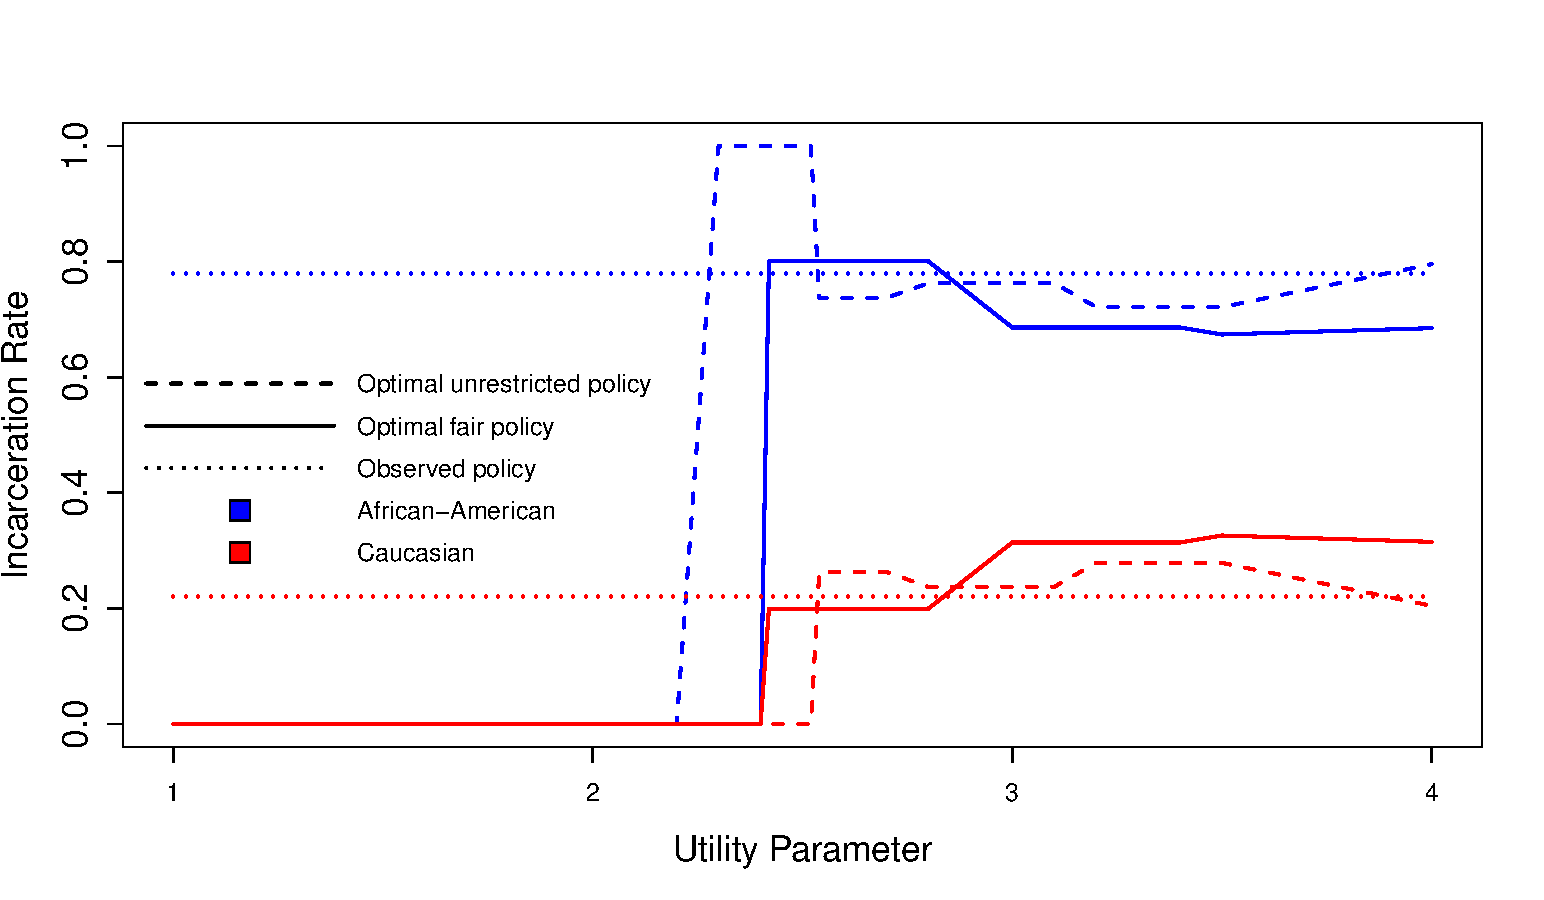
\includegraphics[scale=.32]{GroupRates.pdf}%compas_plot.pdf}
\end{center}
\caption{Group-level incarceration rates %(proportion of individuals with $A=1$) 
	for the COMPAS data as a function of the utility parameter $\theta$.}
\vspace{-4.7mm}
\label{sim}
\end{figure}

\section{Conclusion}
\label{sec:conc}

We have extended a formalization of algorithmic fairness from \citet{NabiShpitser18Fair} to the setting of learning optimal policies under fairness constraints.
%Our approach is tailored for settings where instances are drawn from distributions where fairness criteria are violated, and where distributions over some variables, such as outcomes, are not under the policy-makers' control.  
We show how to constrain a set of statistical models and learn a policy such that
%a high quality policy and a set of constrained statistical models may be learned in such a way that
subsequent decision making given new observations from the ``unfair world'' induces high-quality outcomes while satisfying the specified fairness constraints in the induced joint distribution.  
%This property is maintained on subsequent instances drawn from the observed distribution where these constraints were originally violated.  
In this sense, our approach can be said to ``break the cycle of injustice'' in decision-making.
%, where unfairness is introduced or reinforced by policies that lead to inappropriate dependence between outcomes or decisions and sensitive features such as race or gender.
%We developed three strategies for optimal fair learning, each of which require modeling different components of the likelihood.
We investigated the performance of our proposals on synthetic and real data, where in the latter case we have supplemented the data with a heuristic utility function. 
%Our synthetic experiments illustrate that the three methods are broadly convergent, but exhibit differences which may be exacerbated in applied settings where the different components of the likelihood may be differentially misspecified. Our COMPAS example illustrates the dependence of the outcome on parameters of the presumed utility function. 
In future work, we hope to develop and implement more sophisticated constrained optimization methods, to use information as efficiently as possible while satisfying the desired theoretical guarantee, and to explore nonparametric techniques for complex settings where the likelihood is not known.


% Acknowledgements should only appear in the accepted version.
%\section*{Acknowledgements}
%\textbf{Do not} include acknowledgements in the initial version of the paper submitted for blind review.

\clearpage

\section*{Acknowledgments}
This project is sponsored in part by the National Institutes of Health grant R01 AI127271-01 A1 and the Office of Naval Research grant N00014-18-1-2760. 

{\small

\bibliography{references}
\bibliographystyle{icml2019}
}
\end{document}
